\documentclass[tikz,border=2pt]{standalone}
\usepackage{amsmath,amssymb}
\usepackage{tikz}
\usetikzlibrary{arrows.meta}

\begin{document}
% The angle between x and y is read off the dot product: cos(theta) = x.y / (||x|| ||y||).
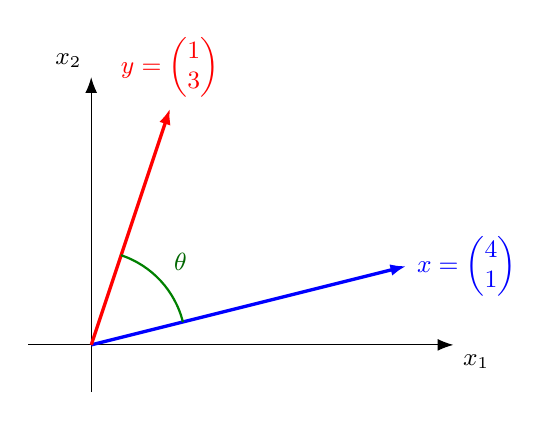
\begin{tikzpicture}[every node/.style={font=\small}, >={Latex[length=2mm]}]
	\draw[->] (-0.8,0) -- (4.6,0) node[below right] {$x_1$};
	\draw[->] (0,-0.6) -- (0,3.4) node[above left] {$x_2$};
	\draw[->, blue, very thick] (0,0) -- (4,1) node[right] {$x=\begin{pmatrix}4\\1\end{pmatrix}$};
	\draw[->, red, very thick] (0,0) -- (1,3) node[above] {$y=\begin{pmatrix}1\\3\end{pmatrix}$};
	\draw[green!50!black, thick] (14:1.2) arc (14:71.6:1.2);
	\node[green!40!black] at (43:1.55) {$\theta$};
\end{tikzpicture}
\end{document}
